% o \label{codigo} serve para podermos fazer referencias para algo numerado, 
% como capitulos, tabelas, figuras, etc. 
% Quando colocamos o comando \ref{codigo}. o compilador troca o \ref{codigo}
% pelo numero atribuido ao \label{}
% ex. \label{tabelaLegal}
%   A tabela \ref{tabelaLegal} mostra que...
% vai ser substituido por
%   A tabela 2 mostra que

\chapter{Desenvolvimento}\label{cap-desenvolvimento}

Segundo o processo iterativo de desenvolvimento descrito na metodologia, 
este projeto evoluiu ao longo de várias etapas de crescente complexidade.


% ---
\section{Objetivo e formulação do problema}\label{sec-objetivos-formulacao-problema}
% ---

Foi inicialmente elaborada uma enunciação geral do problema a ser resolvido: 
a criação de um jogo digital que, valendo-se de técnicas de realidade 
virtual, oferecesse uma experiência imersiva e educativa a crianças de 8 a 12 
anos de idade, de acordo com o recorte selecionado descrito no \autoref{cap-teoria}.
Tendo essa enunciação como base, pôde-se decidir a respeito de restrições, e 
do escopo que guiariam as etapas seguintes de conceituação do projeto.

% ---
\subsection{Ferramentas e tecnologias}\label{subsec-ferramentas-tecnologias}
% ---

Em primeiro lugar, optou-se por restringir os equipamentos e tecnologias a 
serem empregados, de modo a facilitar a acessibilidade e adoção em sala de aula 
e diminuir os custos de implantação, sem que a experiência desejada tivesse de 
ser sacrificada. Isso levou à escolha do uso do \textit{Google Cardboard} 
como dispositivo principal de realidade virtual, por seu baixo custo comparado 
a demais alternativas de mercado, e sua integração a dispositivos móveis que, 
em muitos casos, já estariam ao alcance dos alunos, ou poderiam ser 
providenciados sem um grande impacto orçamentário.

Em adição ao \textit{Cardboard}, optou-se pela implementação do dispositivo 
detector de gestos manuais \textit{Leap Motion} como forma de \textit{input}
principal para o jogo, com a vantagem de ser uma alternativa de custo 
aceitável, capaz de providenciar uma experiência bastante direta na interação 
do aluno com o mundo do jogo, uma vez que permite que movimentos do jogador no 
mundo real sejam traduzidos em ações do mundo virtual, permitindo abstrair os 
dispositivos de entrada e saída por completo, e mantendo a imersão e engajamento.

Por fim, como restrição adicional, a ferramenta \textit{Unity} foi escolhida 
como \textit{engine} de desenvolvimento do jogo, por sua fácil integração 
ao hardware escolhido, e seu paradigma de desenvolvimento em mais alto nível do 
que as demais alternativas disponíveis, o que permitiria ao grupo focar-se 
na conceituação e implementação do jogo em si, sem prender-se a eventuais 
problemas relativos à configuração e uso do hardware, criação de APIs próprias 
ou preocupações com elementos mais elementares da criação de um jogo digital.

% ---
\subsubsection{Alternativas consideradas}
% ---

Alguns outros dispositivos, de função semelhantes aos 
citados anteriormente, foram considerados como potenciais 
alternativas àqueles escolhidos para a realização deste 
trabalho.

Como alternativa para a implementação de controles 
gestuais, considerou-se duas principais alternativas: 
o controlador por infra-vermelho \textit{Leap Motion} 
e o bracelete de controle por contrações musculares 
\textit{Myo}. 

O controlador \textit{Myo}, que funciona medindo a 
contração e o relaxamento de músculos no braço do 
usuário, permitindo detectar gestos e posicionamento 
do braço e das mãos. Sua principal vantagem sobre o 
\textit{Leap Motion} é não estar restrito a uma 
única área de operação: enquanto o \textit{Leap Motion} 
precisa que o usuário mantenha suas mãos dentro da 
área de captura de sua câmera infra-vermelho, o 
\textit{Myo} é capaz de detectar movimentos como 
quer que o usuário se posicione. 

Contudo, este dispositivo apresentou uma série de 
restrições que o apontaram como incompatível com o 
projeto. Primeiramente, enquanto o \textit{Myo} é 
mais adequando que o \textit{Leap Motion} para a 
detecção de gestos maiores, que podem extrapolar 
a restrita área de operação deste, ele é menos 
capaz de detectar gestos finos e, necessários para 
o controle preciso de um jogo nos moldes projetado. 

Além disso o \textit{Myo} tem um custo 
consideravelmente mais elevado que o \textit{Leap Motion}, 
custando USD 199,00 \cite{myo:2016:store} por unidade, 
enquanto o \textit{Leap Motion} está precificado em 
apenas USD 79,99  \cite{leap:2016:store}. Se 
considerarmos que para gestos com duas mãos seriam 
necessários dois braceletes \textit{Myo} por 
usuário, se custo salta então para USD 398,00.

Quanto a dispositivos de realidade virtual, duas 
alternativas ao \textit{Google Cardboard} foram 
trazidas em questão: os \textit{headsets} 
\textit{Oculus Rift} e o \textit{HTC} Vive. 

Dentre estes o \textit{HTC Vive} oferece a 
experiência mais precisa, sendo composto por não 
só um \textit{headset}, mas também sensores 
individuais a serem dispostos pelo ambiente para 
detectar movimentação relativa do jogador. 
Contudo, visto que o jogo contemplado neste projeto 
visa ser aplicável em sala de aula, um equipamento 
que necessite um infra-estrutura tão complexa seria 
incompatível com o que essa estipulação. Há também 
uma incompatibilidade de preços, pois uma unidade de 
\textit{HTC Vive} custaria \$799,00  
\cite{vive:2016:store}, um valor proibitivo para 
uso em larga escala, como pretendido pelo projeto.

O \textit{Oculus Rift}, por outro lado, não 
necessita de sensores externos para operar, 
operando apenas com um \textit{headset}. Apesar 
de sua performance ser superior à do 
\textit{Google Cardboard} - visto que aquele é um 
\textit{hardware} dedicado à realidade virtual 
enquanto este vale-se somente do uso de um celular 
para produzir o efeito tridimensional - o 
\textit{Oculus Rift} ainda possui um preço que 
extrapola o que foi considerado razoável para 
implementação em sala de aula: USD 599,00  
\cite{rift:2016:store} por unidade.

O dispositivo escolhido, o Google Cardboard, pode 
ser adquirido por a partir de USD 15,00  
\cite{cardboard:2016:store}, uma faixa de preço 
muito mais compatível com a ideia original do projeto.

% ---
\subsection{Delimitação do escopo}\label{subsec-delimitacao-escopo}
% ---

Pelo reduzido tempo de execução disponível para a implementação do projeto,
limitada familiaridade com as tecnologias escolhidas, e pelo grupo ser
composto apenas por dois integrantes, decidiu-se manter o escopo do projeto
pequeno, de forma que o grupo pudesse focar-se em criar um jogo que servisse
como prova de conceito, fizesse bom uso da mídia e dos dispositivos empregados,
e implementasse mecânicas diversificadas o suficiente para que testes posteriores
pudessem ser realizados quanto à sua eficácia.

Enquanto não ficaram previamente estipulados em termos específicos a quantidade de
mecânicas a ser implementadas, a extensão do conteúdo criado e a sofisticação
artística pretendida para o produto final, ficou claro que o desenvolvimento do
jogo deveria ser focado na sua realização técnica, e que não seria possível um
alto grau de refinamento e pós-produção equiparável àquele de jogos digitais
disponíveis no mercado. Estas restrições moldaram significativamente as decisões
tomadas durante as etapas posteriores de \textit{brainstorming} e desenvolvimento do
jogo.

% ---
\section{\textit{Brainstorming} e seleção do conceito do jogo}\label{sec-brainstorming-conceito}
% ---

Com a enunciação do problema e as restrições de implementação bem definidas 
e acordadas pelo grupo, pôde-se passar para a etapa seguinte do desenvolvimento, 
o \textit{brainstorm}, durante o qual várias ideias foram debatidas e 
exploradas pelos membros do grupo. Nesta fase, diversas propostas foram feitas 
para uma solução que fizesse um bom uso dos recursos de realidade 
virtual disponíveis e gerasse um projeto adequado ao público alvo 
selecionado, resultando em um jogo intuitivo e divertido que fosse 
capaz de transmitir os conceitos lógicos e cognitivos relevantes.
Importante também era que o jogo exercitasse competências e 
habilidades do raciocínio lógico, apresentados previamente na 
\autoref{quadro:PCN}.

As ideias geradas variaram desde jogos de um ritmo mais acelerado, no qual 
um jogador teria que categorizar elementos abstratos o mais rápido que 
pudesse - segundo características como cor, formato e tamanho - até experiências 
nas quais pressões de tempo e condições de falha estavam completamente 
ausentes, como jogos de resolução de quebra-cabeças tridimensionais, 
e são apresentadas a seguir.

% ---
\subsection{Ideias do brainstorm}\label{subsec-ideias-brainstorm}
% ---

Na \autoref{fig:rascunhos-brainstorm} é possível ver o rascunho das ideias feitas durante o \textit{brainstorm}. 

\begin{figure}[h]
	\centering
	\caption{Primeiro rascunho do jogo}
	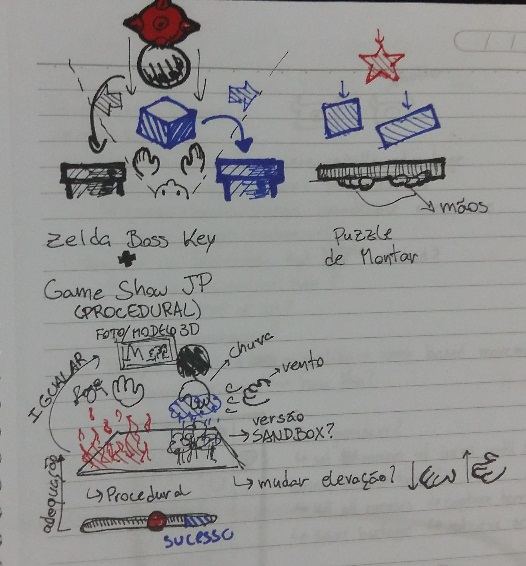
\includegraphics[width=0.5\textwidth]{first_concepts}
	\legend{\fonteAP}
	\label{fig:rascunhos-brainstorm}
\end{figure}

No canto superior direito, vê-se o rascunho de um conceito de jogo aonde 
peças vão caindo lentamente e devem ser empilhadas em uma bandeja ou 
superfície controlada pelo movimento das mãos do jogador, que deve 
movimentar a bandeja de forma que as peças que caem fiquem bem dispostas, 
em vez de tombar para fora da bandeja. Outra possibilidade é que as 
peças caindo tenham que se juntar para fazer um formato específico, 
ou até mesmo uma adaptação do famoso jogo \textit{Tetris}, mas 
tridimensional, aonde deve-se criar um plano inteiro sobre a bandeja 
(ao invés de uma linha, como no jogo original). Esta ideia, além de
exercitar a coordenação motora do jogador, treina também as 
competências e habilidades H1, H2 e H7 do \autoref{quadro:PCN}, pela
necessidade de se resolver o problema atual (de identificar a 
peça que está caindo e aonde ela deve ser colocada), assim como planejar
aonde colocar peças futuras.

No canto superior esquerdo, existe o rascunho de um jogo de 
classificação. Assim como antes, peças vão caindo, e o jogador 
deve categorizar estas peças em uma de duas ou mais categorias, 
através de movimentos das mãos. No exemplo desenhado, o 
objetivo poderia ser mover todos os cubos azuis para a direita, 
esferas pretas para a esquerda, e não agir sobre as esferas 
com espinhos vermelhas. Outras variações poderiam ser feitas, 
também, como todos os cubos (independente de sua cor) vão 
para a direita, por exemplo. Existem inúmeras possibilidades, 
tendo como pré-requisito ser possível categorizar os elementos. 
Adicionalmente, os exemplos dados foram com formas geométricas, 
mas podem ser abstraídas para quase qualquer área, como por 
exemplo elementos (ex. Separe os elementos que reajam com 
oxigênio), geografia (ex. Categorize os países por continente), 
história (ex. Classifique estes eventos como causas ou 
consequências da Segunda Guerra Mundial), ou qualquer outro 
assunto que se consiga imaginar. Esta alternativa pode 
exercitar as competências e habilidades H1, H2, H7 e H8 do 
\autoref{quadro:PCN}, dependendo de quão complexo for o desafio. 
No caso simples de apenas se classificar formas, por exemplo,
apenas a competência H8 será exercitada (além da memória do jogador). Em um caso mais elaborado, 
aonde a ordem em que se colocam elementos em cada uma das categorias 
importe, como por exemplo as peças maiores tem que entrar antes de 
peças menores, as quatro competências listadas podem ser praticadas.

Logo abaixo do rascunho no canto superior esquerdo, estão as 
frases ``Zelda Boss Key'' e ``Game Show JP''. Estas são referências 
para uma terceira ideia de jogo, aonde é apresentado ao jogador 
uma peça tridimensional e uma abertura ou ranhura tridimensional. 
O jogador deve então, com movimentos da mão, rotacionar ou modificar 
a peça para que esta encaixe na ranhura/abertura. Dois exemplos da 
referência do jogo \textit{Legend of Zelda: Skyward Sword} podem 
ser vistos na \autoref{fig:zelda-key-puzzle}, aonde é possivel ver
a peça na frente e, ao fundo, o encaixe. Uma possibilidade mais elaborada 
é possível, aonde, para se encaixar a peça, é necessário uma série 
de movimentos, não apenas uma rotação. Nesta opção, seria possível 
exercitar as competências e habilidades H1, H2 e H8 do 
\autoref{quadro:PCN}, devido à necessidade de se entender a peça 
tridimensional e como ela encaixa na ranhura. Adicionalmente, este 
jogo permitiria melhorar o raciocínio espacial do jogador.

\begin{figure}[h]
	\centering
	\caption{Dois exemplos do \textit{minigame} ``Zelda Boss Key'' do jogo \textit{Legend of Zelda: Skyward Sword}}
	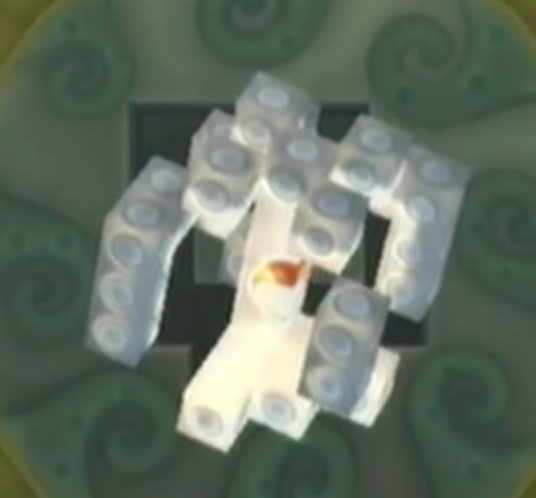
\includegraphics[width=0.3\textwidth]{zelda-puzzle-1}
	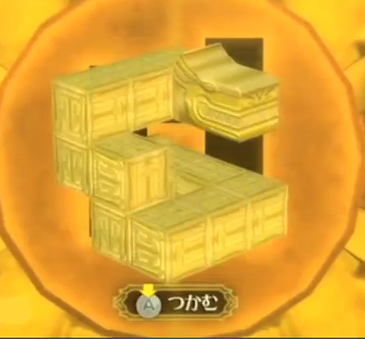
\includegraphics[width=0.3\textwidth]{zelda-puzzle-2}
	\legend{\fontedaimg{\cite{youtube:2016:boss-key}(esquerda) e \cite{zeldainformer:2016:boss-key}(direita)}}
	\label{fig:zelda-key-puzzle}
\end{figure}

Por último, na \autoref{fig:rascunhos-brainstorm}, no canto inferior esquerdo,
é possível ver o rascunho da quarta e última ideia. Neste jogo, os 
jogadores deparariam-se com um terreno digital composto por acidentes
geográficos como planaltos, depressões, corpos d'água e formações magmáticas, 
e poderiam modificá-lo a partir de gestos manuais simples que controlassem 
a elevação, precipitação, movimentação do ar, entre outros. O objetivo do jogo
é manipular a pequena configuração geológica tridimensional, de forma a chegar 
a um determinado estado pré-definido. O terreno seria subdivido em unidades 
cúbicas que poderiam ser manipuladas individualmente, fornecendo uma 
resolução suficiente para que configurações diversas e interessantes pudessem 
ser construídas, mas sem exigir uma precisão incompatível com os dispositivos 
de entrada e saída escolhidos. Esta última alternativa exercita as 
competências e habilidades H1, H2, H6 e H7 do \autoref{quadro:PCN}, dada 
a sua necessidade de solucionar desafios por partes, além de conseguir priorizar e
planejar os movimentos seguintes necessários para se chegar ao estado
pré-definido.

% ---
\subsection{Seleção do conceito do jogo}\label{subsec-selecao-conceito}
% ---

Por fim, uma análise cuidadosa das limitações das tecnologias escolhidas, aliada 
a uma preocupação em manter o jogo intuitivo e imersivo levou o grupo a 
escolher o último conceito dentre os quatro. Os dois primeiros conceitos, por 
mais interessantes que fossem, tinham uma dependência muito forte sobre a
entrada do controlador \textit{Leap Motion}. Dado que o controlador não 
é completamente preciso e poderia falhar na detecção de movimentos ou 
na captura da mão do jogador, era necessário prevenir que o jogador fosse
punido indevidamente.
Visto que os dois primeiros conceitos dependiam dos objetos caindo, 
uma falha do controlador poderia fazê-los perder, causando frustração. 
Entre o terceiro e quarto conceito, o grupo escolheu o último, devido a 
um interesse maior e também pelo número muito maior de 
possibilidades de interações. O jogador possivelmente perderia o interesse no terceiro 
conceito após poucas partidas do jogo.

Desta forma, o quarto conceito foi o escolhido para ser desenvolvido. 
O próximo passo era definir formalmente as mecânicas do jogo, 
assim como os elementos que o jogador poderia manipular. Estes 
elementos estão listados no \autoref{quadro:elementos}, junto das 
interações planejadas para cada um.

\begin{quadro}[htb] 
	\centering
	\caption[Elementos manipuláveis pelo jogador]{Elementos manipuláveis pelo jogador}
	
	\begin{tabular} {| >{\centering\arraybackslash} m{3cm} | m{9cm} |}
		\hline
		%Multicolumn usado só no header para centralizá-lo
		\textbf{Elemento} & \multicolumn{1}{>{\centering\arraybackslash}m{9cm}|}{\textbf{Interação planejada}} \\
		\hline
		Terra/Pedra & O principal elemento do mundo. O jogador consegue manipular os blocos de terra modificando sua altura, criando pilares ou buracos \\
		\hline
		Água & O jogador consegue causar precipitação em uma área pre-determinada, criando corpos d'água, como lagos \\
		\hline
		Fogo & O jogador pode colocar fogo em uma área pre-determinada, secando corpos d'água que estiverem ali \\
		\hline
		Vento & O jogador consegue criar correntezas de vento em uma das quatro direções cardeais. Se aplicados em uma configuração específica dos blocos, o vento cria ondas num corpo d'água que erode um bloco de terra/pedra, criando areia \\
		\hline
		Lava & Esse elemento não pode ser gerado pelo jogador, sendo encontrado no nível mais baixo do mundo em algumas fases. Se um buraco é escavado até este nível mais baixo, a lava começa a subir. Em contato com água, a lava vira terra/pedra \\
		\hline
		Areia & Criado pela erosão de terra/pedra devido à interação do vento com a água \\
		\hline
	\end{tabular}
	
	\legend{\fonteAP}
	\label{quadro:elementos}
\end{quadro}


Para que o jogo não fosse curto demais, foram então imaginados cenários 
que extrapolassem os usos básicos das 
mecânicas propostas, de maneiras que se alinhassem aos conceitos pedagógicos 
que deveriam ser transmitidos pelo jogo: desafios que dependessem da execução 
de tarefas em uma determinada ordem, em combinação com outras tarefas paralelas, 
ou dentro de um determinado limite de tempo. Nestes cenários, era esperado 
que jogadores conseguissem imaginar soluções mais sofisticadas, indo além 
das interações básicas às quais teriam acesso direto. Seria necessário 
movimentar massas de ar para jogar água contra blocos de terra (cujo rascunho 
é mostrado na \autoref{fig:rascunhos-praia}), formando 
praias; escavar o solo para alcançar câmaras magmáticos e formar vulcões; ou 
alterar o curso de corpos d'água para formar cascatas.

\begin{figure}[htb]
	\centering
	\caption{Rascunho de como criar uma praia, utilizando os elementos terra, água e ar}
	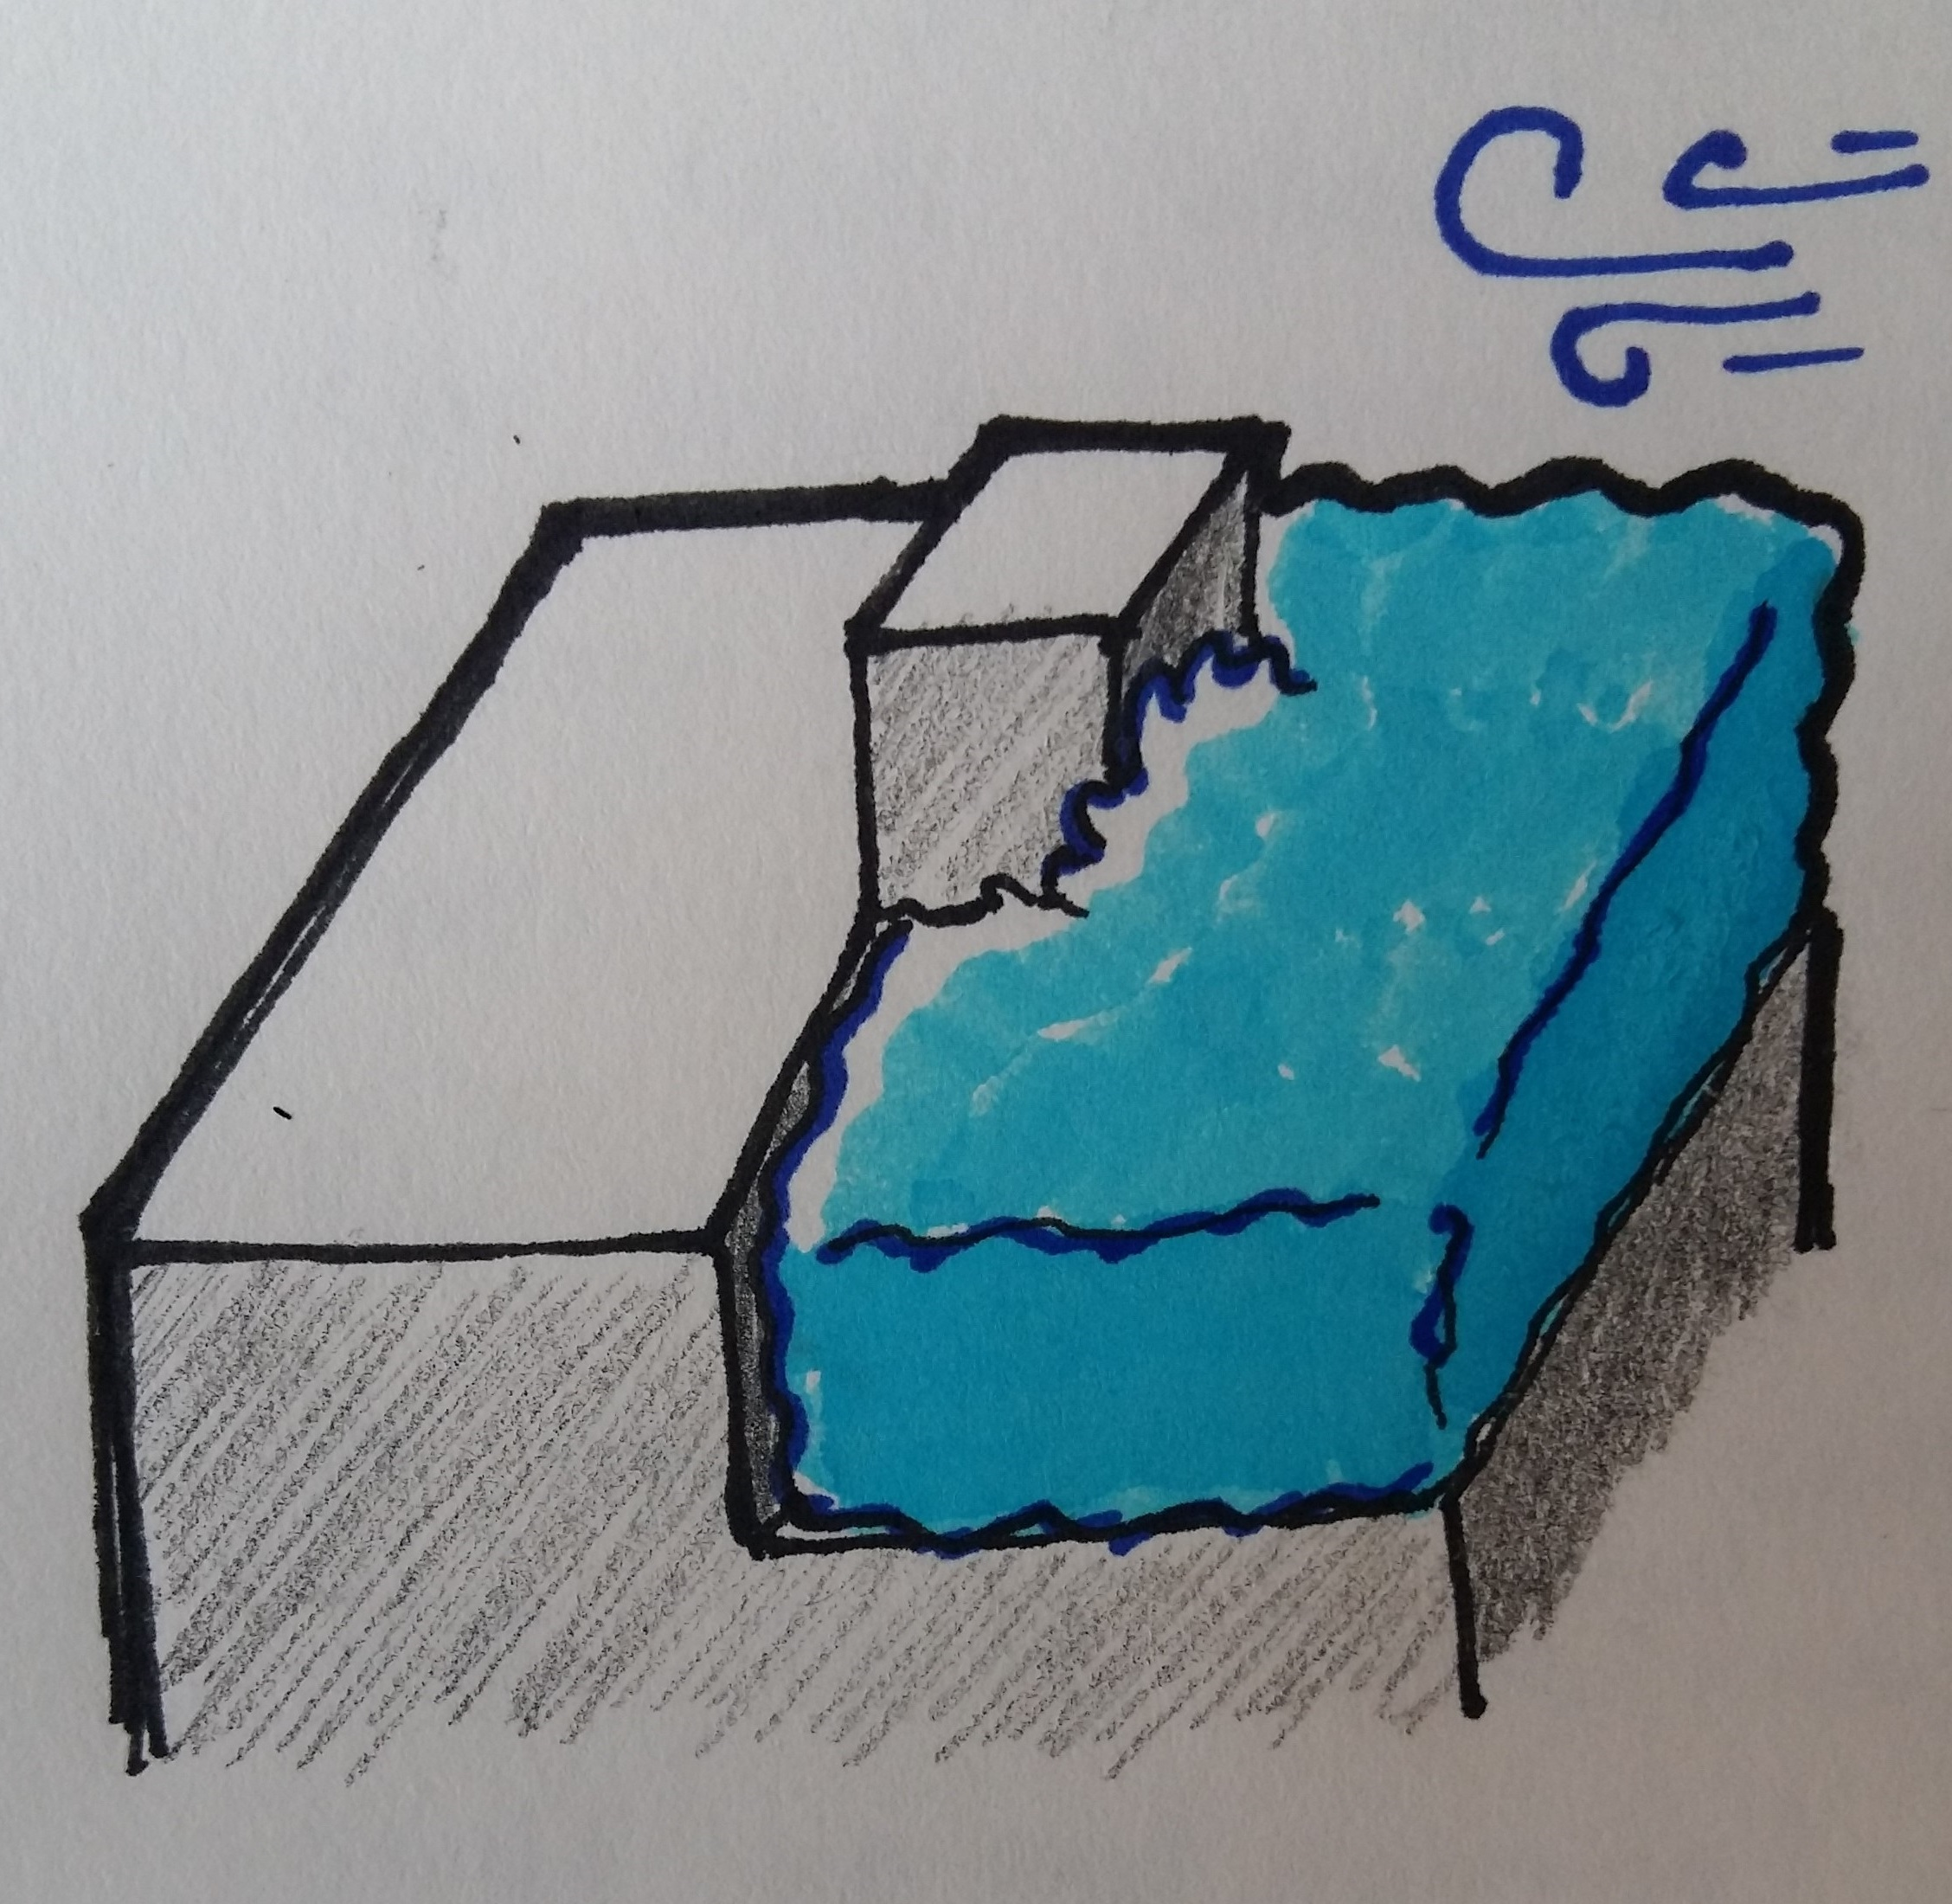
\includegraphics[width=0.5\textwidth]{draft2}
	\legend{\fonteAP}
	\label{fig:rascunhos-praia}
\end{figure}

Algumas primeiras ideias de possíveis fases também foram discutidas, para 
dar uma direção para a criação da prova de conceito. A primeira fase lidaria 
apenas com a mudança da elevação da terra e o jogador teria que criar um 
buraco e uma torre de terra, algo similar à \autoref{fig:rascunho-torre-buraco}.
Desta forma, a primeira prova de conceito já poderia ser jogada 
para se testar a viabilidade do conceito.

\begin{figure}[ht]
	\centering
	\caption{Rascunho de uma possível primeira fase}
	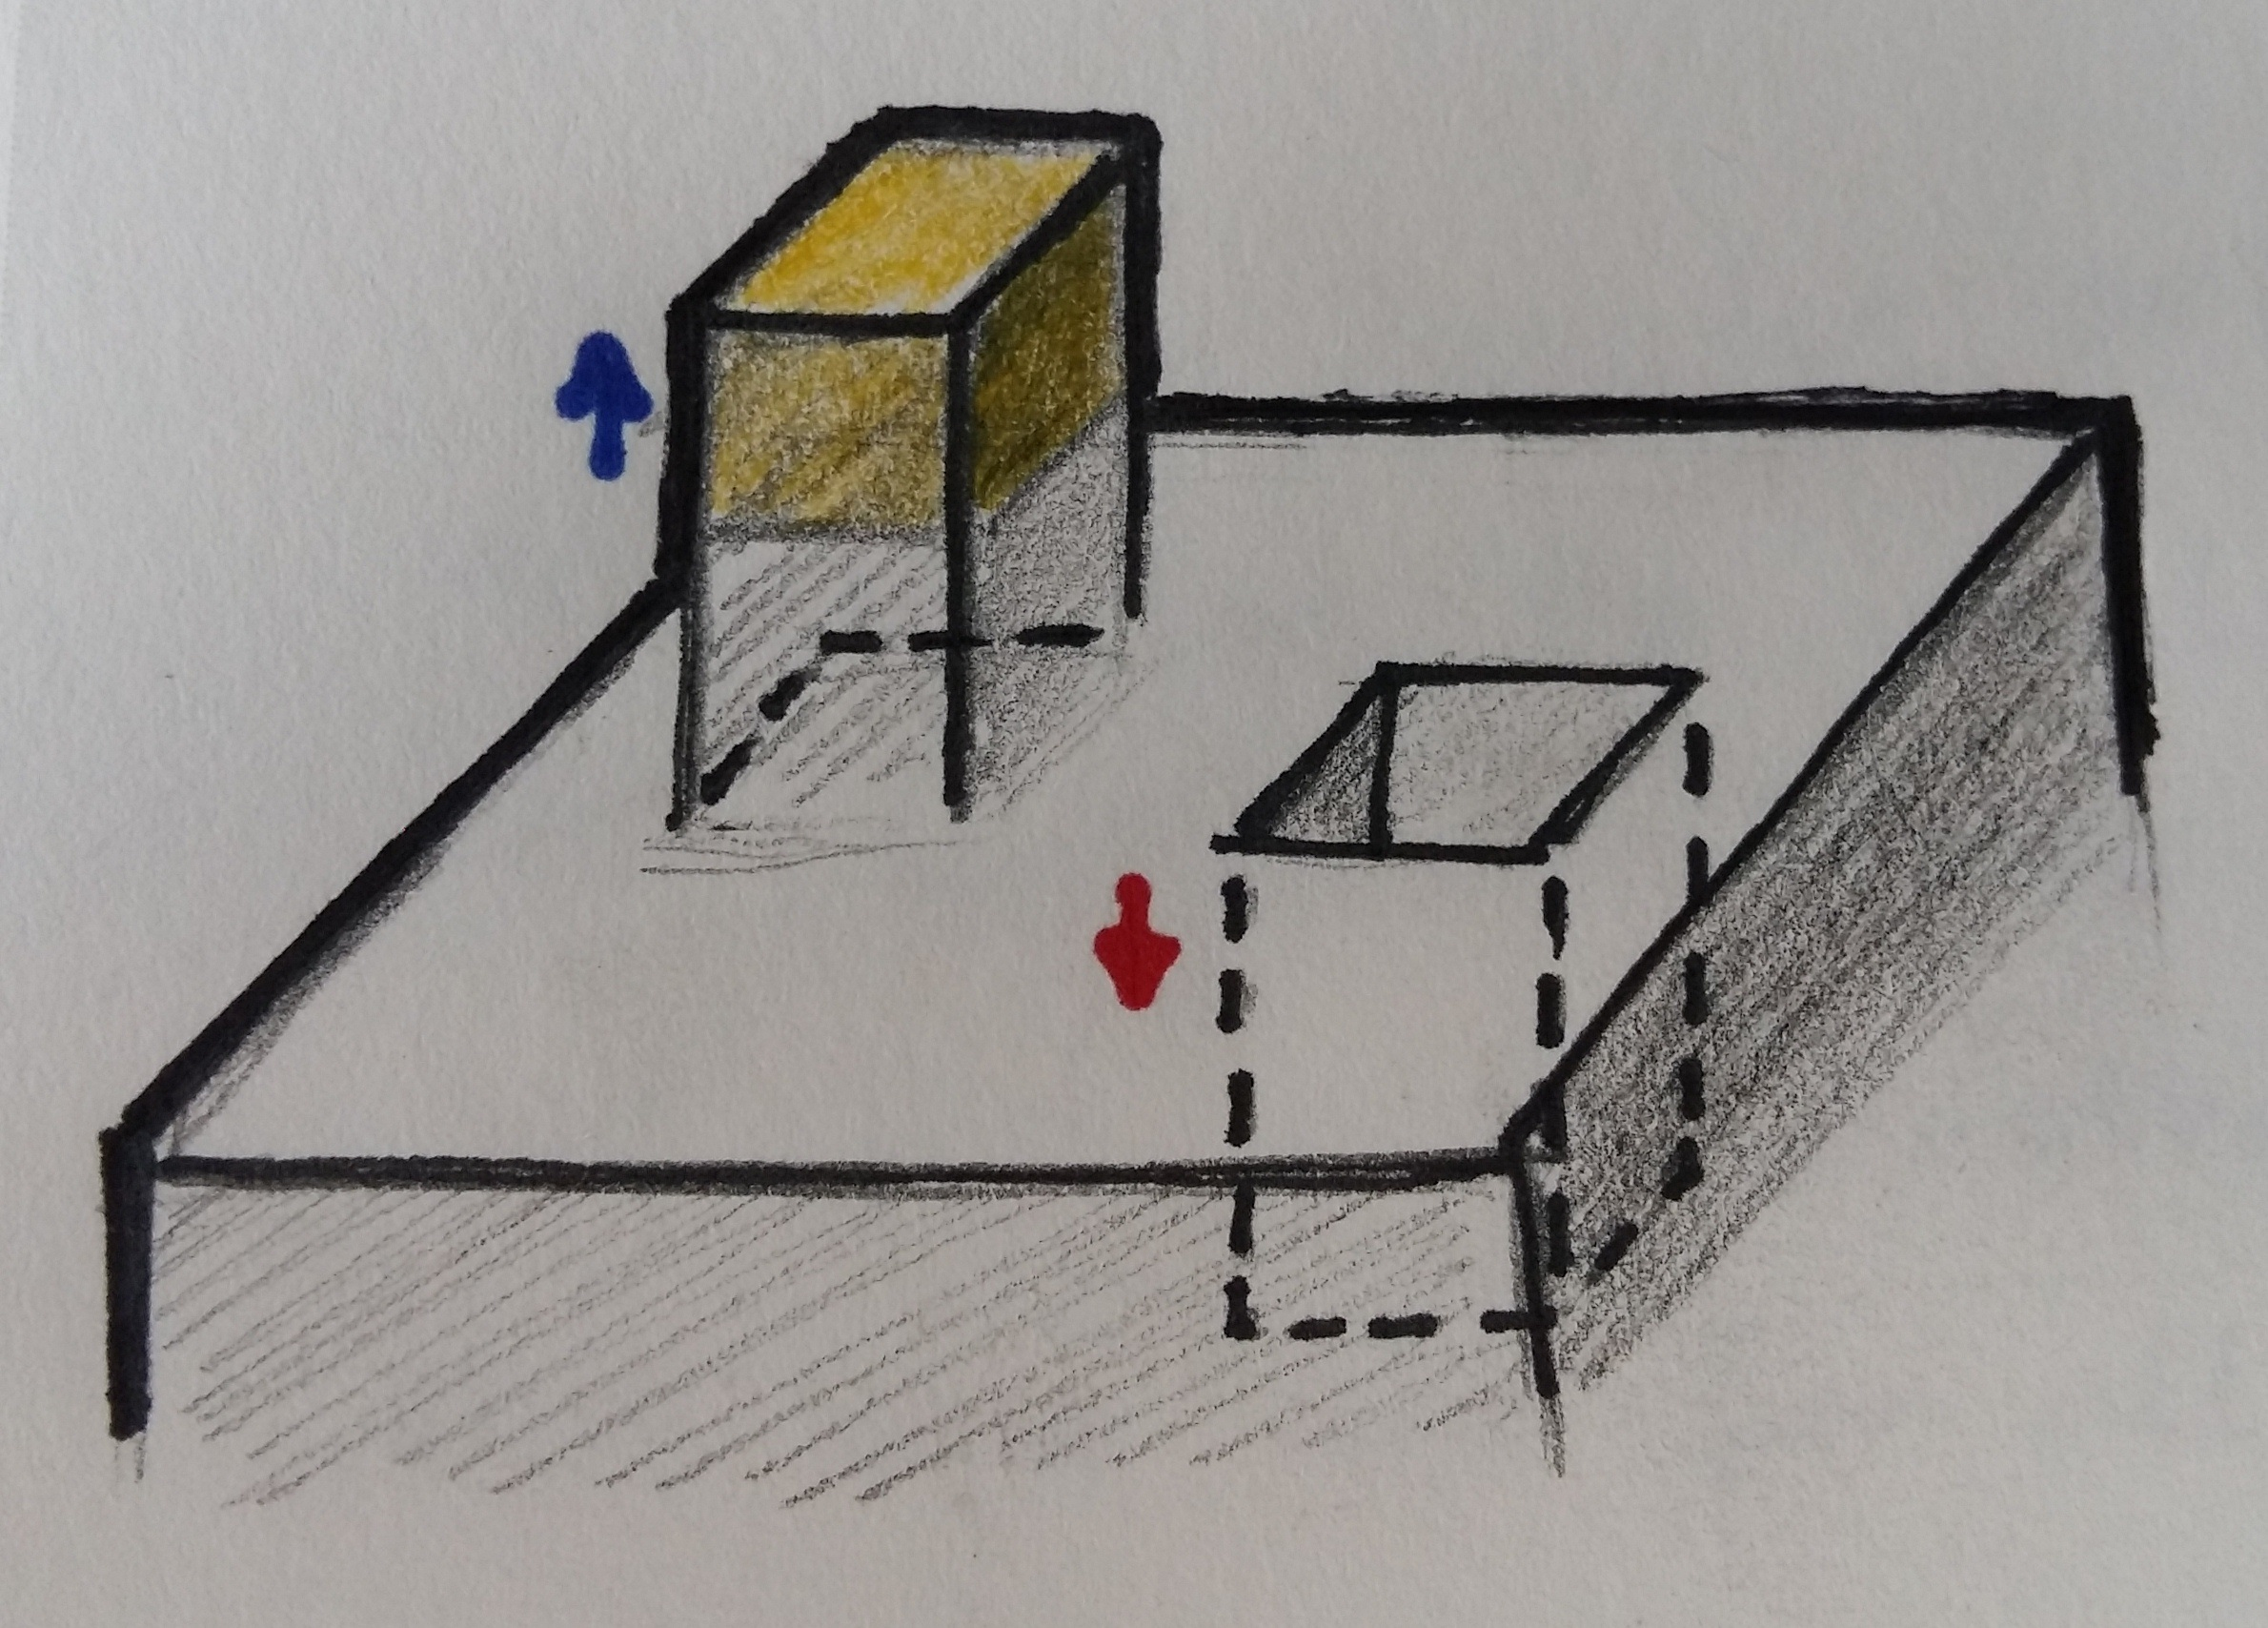
\includegraphics[width=0.5\textwidth]{draft1}
	\legend{\fonteAP}
	\label{fig:rascunho-torre-buraco}
\end{figure}

Uma vez escolhido o conceito do jogo, pode-se iniciar o 
\textit{GDD}, que deve ser atualizado conforme o jogo 
evolui. O \textit{GDD} pode ser encontrado no \autoref{apendice:gdd}.

% ---
\section{Primeira iteração: prova de conceito}\label{sec-primeira-iteracao-prova-conceito}
% ---

Uma vez decidido o conceito a ser explorado, um pequeno protótipo foi proposto 
para dar ao grupo uma noção mais palpável de como esse jogo se pareceria, como 
seria controlá-lo, que dificuldades imprevistas apareceriam e quais as medidas 
que precisariam ser tomadas para suplantá-las. Este protótipo inicial tinha 
como objetivo tanto familiarizar o grupo às ferramentas e tecnologias 
escolhidas para a realização do trabalho quanto ajudar a nivelar de maneira 
mais concreta a complexidade de sua implementação.

O protótipo deveria se ater apenas a uma mecânica básica da especificação 
do conceito: controle da elevação do terreno. O jogador teria acesso direto ao 
jogo - sem passar por telas de menu ou tutoriais - no qual se depararia com 
uma grade tridimensional de 5x5x5 cubos de terra, os quais poderia elevar 
ou rebaixar livremente. Um exemplo desta prova de conceito está 
demonstrado na \autoref{fig:primeiro-screenshot-terra}.

\begin{figure}[h]
	\centering
	\caption{Prova de conceito do jogo}
	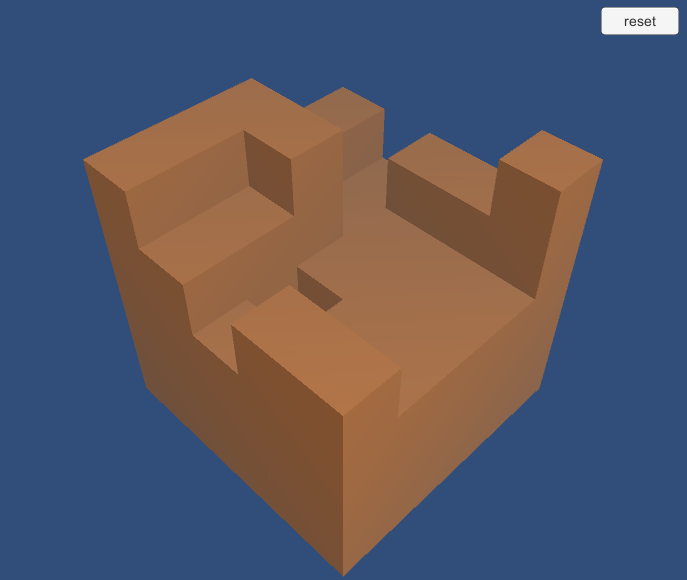
\includegraphics[width=0.5\textwidth]{ss1}
	\legend{\fonteAP}
	\label{fig:primeiro-screenshot-terra}
\end{figure}

Apesar da simples implementação, algumas primeiras dificuldades já puderam 
ser percebidas nesta iteração, sobretudo na integração dos dispositivos de 
realidade virtual.

A primeira barreira a ser percebida foi a falta de compatibilidade com 
dispositivos \textit{Android} da versão mais recente do \textit{SDK} do 
controlador \textit{Leap Motion}, como havia nas versões anteriores. Isso, aliado 
ao fato de que a versão anterior do \textit{SDK} não estava mais disponível 
para download, significou que uma interação direta entre o \textit{Leap Motion} 
e o jogo compilado para dispositivos móveis não seria possível nessa etapa 
inicial do projeto. A solução para este problema foi continuar o desenvolvimento
diretamente no computador, sem se preocupar em gerar a versão para o 
\textit{Android} (e, portanto, para o \textit{Google Cardboard}).

Apesar deste empecilho, \textit{Unity} se mostrou uma plataforma robusta e 
flexível o suficiente para a continuação do projeto, e as mecânicas básicas 
puderam ser implementadas rapidamente e sem grandes problemas.

% ---
\section{Segunda iteração: mecânicas básicas}\label{sec-segunda-iteracao-mecanicas-basicas}
% ---

Tendo em mente as facilidades e desafios percebidos durante a criação da prova 
de conceito, um segundo protótipo foi desenvolvido, desta vez com o intuito 
de acrescentar uma segunda mecânica básica - controle da precipitação - de modo
a permitir que o jogador experimentasse com a interação entre as duas.

Para tal, foi necessário especificar um pouco melhor a mecânica da água 
e como ela funcionaria em relação às mudanças de altura do terreno. 
Primeiro, definiu-se que a agua deveria crescer de baixo para cima, de
maneira similar a um recipiente sendo preenchido com líquido, demonstrado
na \autoref{fig:mecanica-agua-enchendo-graficamente}. Esta era uma
definição mais referente ao apelo gráfico do que uma mecânica. Adicionalmente, 
definiu-se que, dado um bloco (ou conjunto de blocos) selecionados, a ação de
precipitação preencheria o espaço aberto até cobrir os blocos selecionados, em 
vez de preencher de água para que esta fique no mesmo nível do bloco selecionado.
Esta mecânica pode ser vista na \autoref{fig:mecanica-agua-enchendo-mecanica}.

\begin{figure}[ht]
	\centering
	\caption{Mecânicas da água 1}
	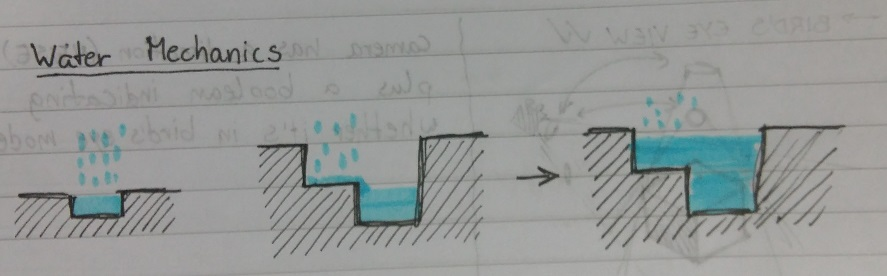
\includegraphics[width=0.5\textwidth]{water_mechanics1}
	\legend{\fonteAP}
	\label{fig:mecanica-agua-enchendo-graficamente}
\end{figure}

\begin{figure}[ht]
	\centering
	\caption{Mecânicas da água 2}
	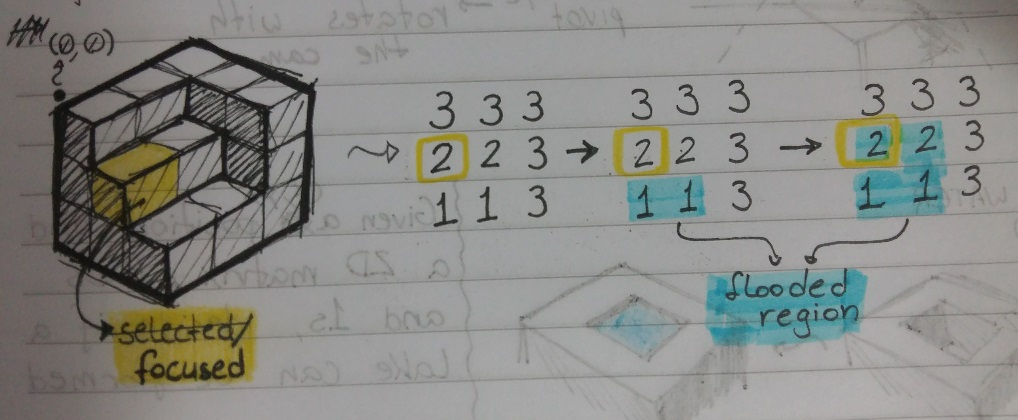
\includegraphics[width=0.5\textwidth]{water_mechanics2}
	\legend{\fonteAP}
	\label{fig:mecanica-agua-enchendo-mecanica}
\end{figure}

Nesta iteração, haveria dois gestos que deveriam ser captados e interpretados 
pelo \textit{Leap Motion}: abaixar e elevar a mão com a palma aberta para alterar 
a elevação do terreno e apontar todos os dedos para baixo para fazer chover em 
uma área específica.

Durante a implementação dessas mecânicas, ficou clara a necessidade de uma 
mecânica de seleção que permitisse a manipulação de grandes áreas do terreno
simultaneamente, então um terceiro gesto foi adicionado: pinçar e arrastar 
para delimitar áreas.

Também nessa etapa, percebeu-se que, devido à posição do \textit{Leap Motion},
alguns dos gestos imaginados para as diferentes mecânicas do jogo - sobretudo 
o associado a chuva - não poderiam ser captados com a precisão necessária, 
obrigado o grupo a reimaginar uma parte significativa da interação. Isto 
resultou na simplificação do gesto para a chuva, bastando apenas fechar o punho
com a palma virada para baixo. Desta forma, o gesto era capturado mais facilmente,
mas também era ativado muitas vezes quando o jogador não havia feito o gesto, 
dificultando a jogabilidade. Uma possível razão para isto é ter definido o 
gesto de maneira não ótima, devido à inexperiência neste assunto por parte
dos integrantes do grupo.

Apesar de tudo, o protótipo já estava jogável e era possível modificar 
o terreno e adicionar ou remover água, como mostrado 
na \autoref{fig:example-water-earth}.

\begin{figure}[ht]
	\centering
	\caption{Prova de conceito do jogo}
	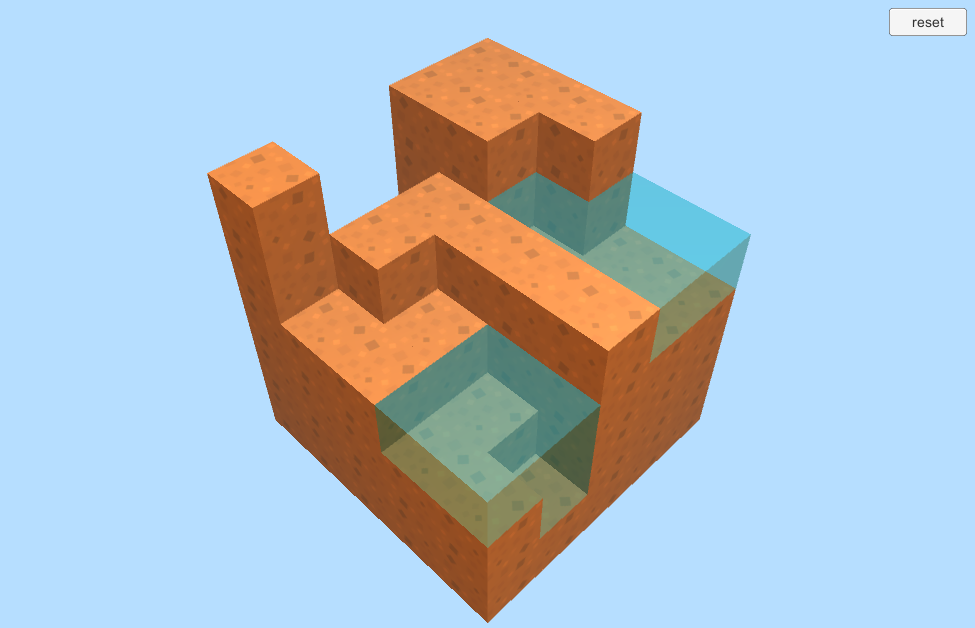
\includegraphics[width=0.5\textwidth]{ss2}
	\legend{\fonteAP}
	\label{fig:example-water-earth}
\end{figure}

% ---
\section{Terceira iteração: últimas mecânicas}\label{sec-terceira-iteracao-ultimas-mecanicas}
% ---

Ao final da segunda iteração, faltavam dois elementos para
completar o conjunto de elementos que o jogador poderia criar, de acordo
com o que havia sido definido: ar/vento e fogo.

O primeiro é importante para permitir a criação de fases que necessitem uma 
sequência maior de passos para se chegar ao objetivo e, portanto, criar
um desafio maior. Já o segundo é importante por sua reação com a água, 
que até então, quando criada, não podia ser removida. Desta forma, o 
fogo serve para desfazer movimentos errôneos de água. Dada a certa 
imprecisão existente com o gesto de geração de água, aonde o nosso
código acusava o jogador de ter feito o gesto erroneamente, o fogo era
importante para minimizar a frustração do jogador.

% ---
\section{Quarta iteração: refinamentos}\label{sec-quarta-iteracao-integracao}
% ---

Uma vez que os elementos principais foram implementados e o jogo já podia
ser jogado, focou-se em possibilitar a execução do jogo no dispositivo \textit{Android}
(que estava, até então, rodando no computador, por dificuldades 
discutidas na \autoref{sec-primeira-iteracao-prova-conceito}). Visto que
a primeira opção, que parecia a mais óbvia, não funcionaria, foi feito um 
estudo mais a fundo sobre a arquitetura do sistema, que está descrita
na \autoref{sec-desenvolvimento-arquitetura}. 

Adicionalmente, erros de código foram corrigidos, e melhorias foram
feitas na detecção de gestos.

% ---
\section{Requisitos}\label{sec-requisitos}
% ---

Os requisitos a seguir foram especificados a partir do \textit{GDD}.

% ---
\subsection{Requisitos não funcionais}\label{subsec-requisitos-nao-funcionais}
% ---

\begin{alineas}
	\item o sistema de reconhecimento de gestos deve tolerar variações 
	 de velocidade, ângulo e posição das mãos para aumentar a taxa 
 	 de reconhecimento dos movimentos executados pelo jogador. Os 
	 valores de tolerância serão testados e selecionados para maximizar 
	 a usabilidade e a experiência do usuário;
	\item o aplicativo deve ser compatível com \textit{Android} 4.4
	 (\textit{KitKat}) em diante, por se tratar de 83.5\% dos 
	 dispositivos \textit{Android}, de acordo com 
	 \cite{google:2016:androidVersion}.
	
\end{alineas}


% ---
\subsection{Requisitos funcionais}\label{subsec-requisitos-funcionais}
% ---

\begin{alineas}
	\item o jogador deve poder interagir com o ambiente do jogo 
	 por meio de gestos predefinidos;
	\item o jogo deve conter os elementos água, fogo,
	 terra e ar;
	\item deve ser possível selecionar 
	 uma área do mundo com a qual se deseja interagir;
	\item o início do jogo deve ser focado em ensinar ao
	 jogador as mecânicas básicas e as interações entre os elementos;
	\item as fases do jogo devem ter sua complexidade aumentada
	 gradativamente, envolvendo cada vez mais mecânicas e
	 interações entre elementos;
	\item algumas fases devem apresentar desafios que envolvam
	 não apenas a escolha adequada de mecânicas e interações, 
	 mas também a escolha da ordem em que eles devem ser aplicados;
	
	\item deve ser possível jogar com o modo de realidade virtual
	 desligado, para os casos aonde o jogador sinta náusea 
	 devido ao \textit{headset}; 
	\item o mundo deve ser discreto, dividido em blocos bem
	 definidos, que podem ser selecionados e modificados.	
\end{alineas}

% ---
\section{Arquitetura}\label{sec-desenvolvimento-arquitetura}
% ---

Para se definir a arquitetura do sistema, é antes necessário identificar e 
entender cada um dos principais elementos, assim como suas interfaces.

% ---
\subsection{Identificação dos elementos}\label{subsec-identificacao-elementos}
% ---

% ---
\subsubsection{Controlador \textit{Leap Motion}}\label{subsubsec-elemento-leapmotion}
% ---

Conforme visto na Seção \ref{subsec-teo-leap-motion}, o controlador pode 
ser dividido em dois elementos diferentes: O \textbf{hardware do controlador} e 
o \textbf{serviço} que aplica algoritmos de visão computacional nas imagens 
vindas do hardware, transformando-as em dados estruturados.

O serviço pode ser executado no computador ou, no caso de se utilizar a versão 
v2 do \textit{SDK} do \textit{Leap Motion}, no \textit{Android}.

% ---
\subsubsection{Lógica do jogo}\label{subsubsec-elemento-logica-jogo}
% ---

Este é o elemento que age sobre o ambiente virtual a partir de dados de entrada 
do controlador e do movimento do \textit{headset} de realidade virtual. 
Este elemento estará implementado no \textit{Unity}, e pode ser executado ou no 
computador ou no próprio celular.

% ---
\subsubsection{Processamento de saída do video}\label{subsubsec-elemento-video}
% ---

Este elemento é controlado pelo \textit{SDK} do \textit{Google Cardboard} e 
cuida de toda a parte de gerar a visão estereoscópica necessária para a visão 
3D, além de movimentar a visão do jogo de acordo com o movimento do 
\textit{headset} de realidade virtual. Este elemento pode ser executado ou 
no computador ou no próprio celular.

% ---
\subsection{Arquiteturas estudadas}\label{subsec-arquiteturas-estudadas}
% ---

As três arquiteturas estudadas têm como entrada as imagens vindas do 
controlador \textit{Leap Motion} e do movimento do \textit{Google Cardboard}, 
que são enviadas à lógica de jogo que, então, modifica o estado do jogo e envia 
para o \textit{Google Cardboard}. As diferentes opções de arquitetura diferem 
quanto à como a conexão é feita, se é intermediada ou não por um computador, e 
aonde essa intermediação acontece.

% ---
\subsubsection{Alternativa utilizando o servidor \textit{WebSocket}}\label{subsubsec-arquiteturas-leapmotion-pc-leapdata-android}
% ---

Nesta opção, conecta-se o controlador a um computador que esteja rodando o 
serviço do \textit{Leap Motion}, transformando as imagens do controlador em 
dados estruturados. O celular que está executando a lógica do jogo então se
conecta ao servidor \textit{websocket} gerado pelo serviço do controlador que 
esta rodando no computador. A partir desta conexão, o servidor envia os
dados estruturados ao celular para que estes possam ser utilizados como 
entradas no jogo. O celular então aplica as transformações necessárias para 
a saída de vídeo, que é enviada à tela do celular.
Esta opção é demonstrada na \autoref{fig:arquitetura-leap-pc-leapdata-android}.

\begin{figure}[ht]
	\centering
	\caption{Alternativa de arquitetura com servidor WebSocket}
	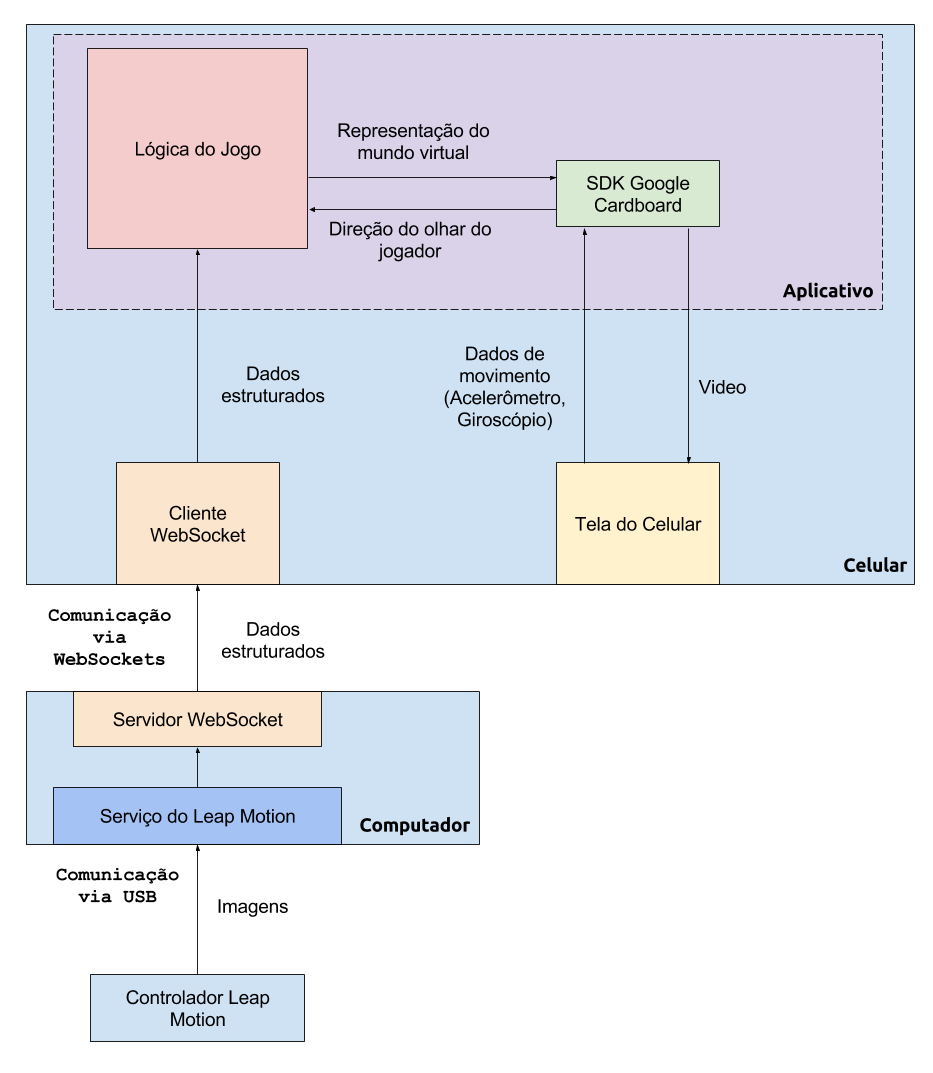
\includegraphics[width=0.7\linewidth]{images/Arquitetura-leap-pc-leapdata-android}
	\legend{\fonteAP}
	\label{fig:arquitetura-leap-pc-leapdata-android}
\end{figure}

A vantagem desta opção é que podemos utilizar a versão mais recente 
do \textit{SDK} do \textit{Leap Motion}, que melhorou muito o rastreamento das 
mãos, comparada à versão v2. Adicionalmente, o serviço já expõe uma interface 
web para a leitura dos dados estruturados. 

Uma desvantagem desta opção, porém, é a necessidade de modificar a biblioteca 
do \textit{Leap Motion} do \textit{Unity} para que esta aceite conexões web, já 
que, nativamente, ela aceita apenas conexões via USB. Outra desvantagem é a 
latência adicionada entre o movimento das mãos do usuário e o momento em que 
a lógica do jogo recebe tais informações. Se esta latência for alta demais, 
cria-se uma dissociação entre a mão do jogador e a mão virtual, 
diminuindo a imersão no jogo.

% ---
\subsubsection{Alternativa com \textit{streaming} do video}\label{subsubsec-arquiteturas-leapmotion-pc-riftcat-android}
% ---

O diferencial desta opção é que a lógica do jogo roda no computador, e a saída 
de vídeo é transmitida para o celular via algum software, como o Riftcat(pago) ou
o TrinusVR(gratuíto). Desta forma, o controlador é conectado diretamente 
ao computador, que está rodando o serviço do \textit{Leap Motion} e lê 
diretamente dele os dados estruturados. Esta arquitetura pode ser vista 
na \autoref{fig:Arquitetura-leap-pc-riftcat-android}.

\begin{figure}[ht]
	\centering
	\caption{Alternativa de arquitetura com streaming do video}
	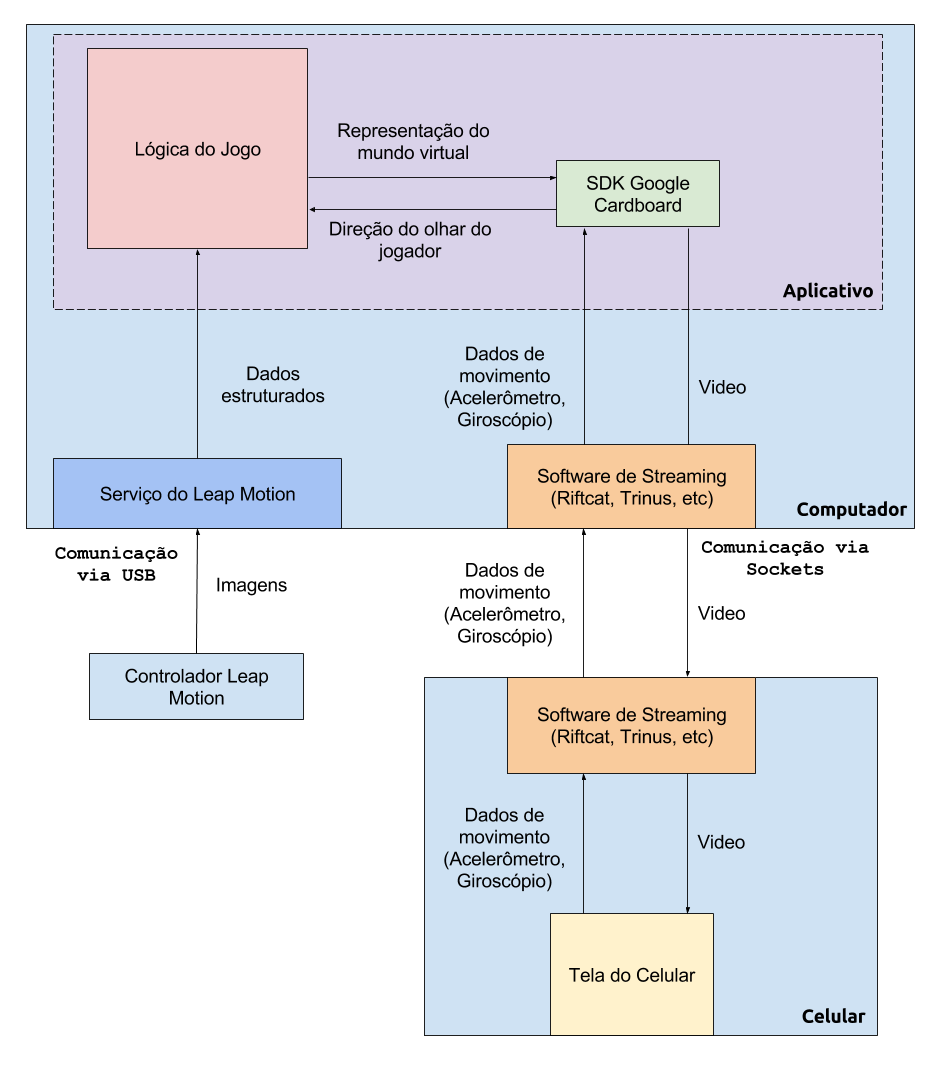
\includegraphics[width=0.7\linewidth]{images/Arquitetura-leap-pc-riftcat-android}
	\legend{\fonteAP}
	\label{fig:Arquitetura-leap-pc-riftcat-android}
\end{figure}

A vantagem desta opção é que, por rodar num computador, o poder de 
processamento é mais alto e, portanto, existem mais possibilidades quanto
a algoritmos utilizados, mecânicas do jogo e processamento gráfico. A conexão 
com o controlador, por ser direta, também significa uma latência baixa 
neste quesito. 

O principal contraponto desta opção é o aumento da latência entre o movimento 
da cabeça do usuário e o movimento da cabeça virtual. Esta latência é maior do 
que a da primeira opção pois é necessário enviar os dados referentes ao movimento 
da cabeça do celular para o computador, que então deve enviar as imagens de 
volta para o celular. Essa latência adicional não apenas cria uma dissociação 
entre o jogador e o mundo virtual, mas também pode causar tontura e enjoo.
Adicionalmente, mesmo a latência entre o movimento das mãos do jogador e
sua detecção pelo código sendo baixa, a latência adicionada na saída de vídeo
pode fazer com que pareça que as mãos estejam sendo detectadas com uma latência 
mais alta.

% ---
\subsubsection{Alternativa com conexão direta}\label{subsubsec-arquiteturas-leapmotion-android}
% ---

Nesta opção, o controlador é conectado diretamente ao celular, conforme 
mostrado na \autoref{fig:arquitetura-leap-android}. Desta forma, esta opção 
provê a maior mobilidade e tem o menor número de subsistemas diferentes. Para 
tal, é necessário utilizar o serviço do \textit{Leap Motion} v2 específica para 
o \textit{Android}. Neste caso, todo o processamento é feito diretamente no 
celular (A transformação das imagens em dados estruturados, a lógica do jogo e 
as transformações necessárias para a saída de vídeo). Por esta razão, esta é a 
opção que adiciona a menor latência, devido à inexistência de conexões extras 
entre um computador e o celular, como nas outras opções.

\begin{figure} [ht]
	\centering
	\caption{Alternativa de arquitetura com conexão direta}
	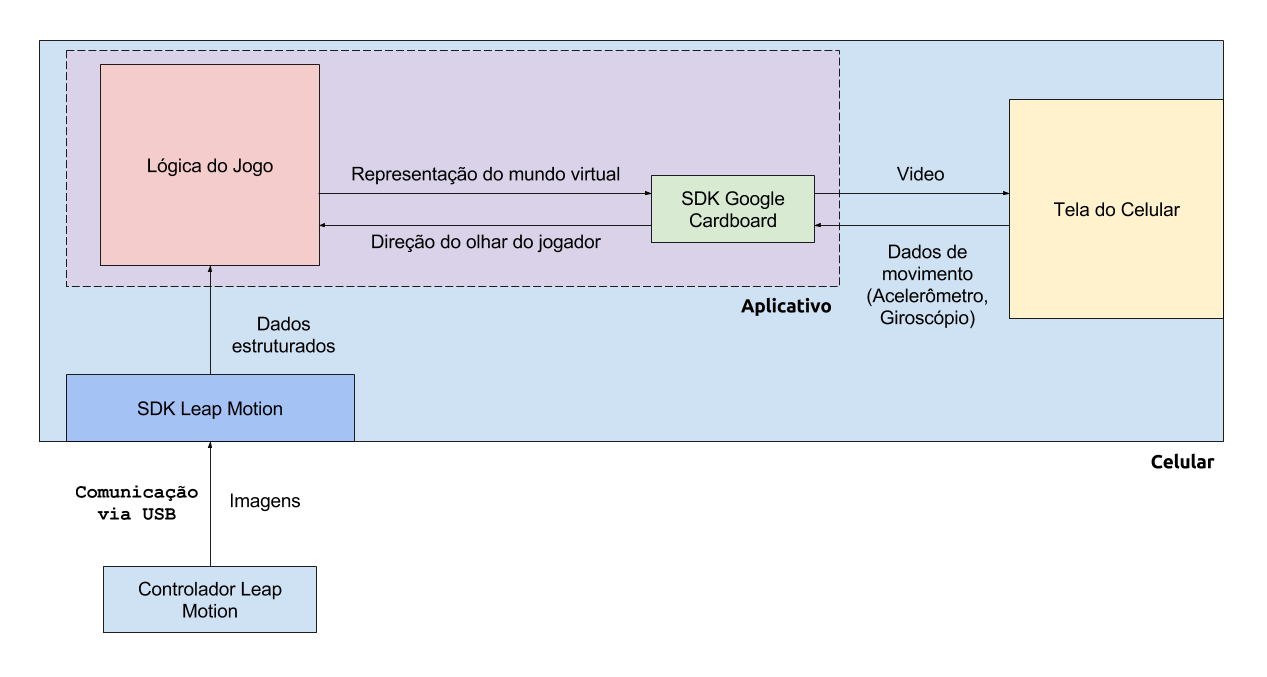
\includegraphics[width=0.7\linewidth]{images/Arquitetura-leap-android}
	\legend{\fonteAP}
	\label{fig:arquitetura-leap-android}
\end{figure}

As desvantagens, porém, são a dependência do serviço do \textit{Leap} nativo 
do \textit{Android}, que estava na versão beta antes de ser descontinuado, e 
também o fato de se tratar da versão v2, que tem um rastreamento pior.

% ---
\subsubsection{Comparação das alternativas}\label{subsubsec-arquiteturas-comparacao}
% ---

A comparação das alternativas pode ser vista no \autoref{tabela:alternativas-arquiteturas}.

\begin{quadro}[htb] \scriptsize
	\centering
	\caption[Comparação das alternativas de arquitetura]{Comparação das alternativas de arquitetura}
		
	\begin{tabular}{|>{\centering\arraybackslash}m{2.1cm}|>{\centering\arraybackslash}m{6cm}|>{\centering\arraybackslash}m{6cm}|}
		\hline 
		\textbf{Alternativa} & \textbf{Pros} & \textbf{Contras} \\
		\hline 
		Servidor Websocket
		&\begin{itemize}[label={},leftmargin=1mm]
			\item Versão mais recente do \textit{SDK} do \textit{Leap}.
			\item Servidor \textit{WebSocket} já disponível com o serviço \textit{Leap Motion}.
		\end{itemize}
		&\begin{itemize}[label={},leftmargin=1mm]
			\item Maior latência entre o movimento da mão e da mão do jogador, pode diminuir imersão.
			\item Necessidade de modificação da biblioteca do \textit{Leap} no \textit{Unity}.
		\end{itemize}
		\\ \hline 
		\textit{Streaming} de Video
		&\begin{itemize}[label={},leftmargin=1mm]
			\item Versão mais recente do \textit{SDK} do \textit{Leap}.
			\item Processamento feito no computador
			\item Conexão direta da lógica do jogo com controlador
		\end{itemize}
		&\begin{itemize}[label={},leftmargin=1mm]
			\item Latência entre movimento da cabeça do jogador e movimento da cabeça virtual, podendo causar desconforto e náusea.
			\item Dependência de mais software, podendo ser pago, e que pode ter como requisito um hardware mais caro para funcionar.
		\end{itemize}
	    \\ \hline 
		Conexão Direta
		&\begin{itemize}[label={},leftmargin=1mm]
				\item Menor latência dentre as opções
				\item Maior mobilidade
				\item Não depende de um computador
			\end{itemize}
		&\begin{itemize}[label={},leftmargin=1mm]
				\item Utiliza a versão v2 do \textit{SDK} do \textit{Leap}, que tem precisão pior.
				\item Necessita da versão beta do serviço para o \textit{Android}, de difícil acesso.
			\end{itemize}
		\\ 
		\hline 
	\end{tabular} 

	\legend{\fonteAP}
\label{tabela:alternativas-arquiteturas}
\end{quadro}

É possivel ver que as alternativas que não têm a conexão direta 
introduzem latências no sistema, mas em locais diferentes. 
O servidor \textit{Websocket} introduz latência na entrada 
referente ao movimento das mãos, enquanto o \textit{streaming} 
de video adiciona atrasos na saída do vídeo para o \textit{headset}. 
Por outro lado, a alternativa da conexão direta utiliza uma 
versão anterior do \textit{SDK} do controlador, que tem um 
rastreamento pior.

% ---
\subsection{Escolha da arquitetura}\label{subsec-arquitetura-escolha}
% ---

Inicialmente, havia se optado pela alternativa da conexão direta. Porém, devido
a impossibilidade de se utilizar a versão \textit{Orion} do \textit{SDK} do 
\textit{Leap Motion}, foi necessário mudar de alternativa. A segunda alternativa 
escolhida foi a do \textit{streaming} de video, visto que a 
sua implementação não necessitaria de mudanças no código. Bastaria gerar 
o executável do jogo no Windows e rodar um software de \textit{streaming}, como o 
Riftcat. Esta alternativa foi testada por um tempo, aonde se constatou
alguns defeitos, como a necessidade de se reiniciar o software várias vezes 
devido a bugs e falta de documentação do Rifcat. Mesmo assim, devido a facilidade
de implementação e qualidade aceitável da solução, a alternativa foi escolhida
como a que seria utilizada.

Porém, descobriu-se posteriormente, ao se testar o software nos computadores
dos outros membros do grupo, que para que esta alternativa funcionasse, 
era necessário uma placa de video relativamente potente, de acordo com 
as especificações mínimas do software, encontrada em
\cite{riftcat:2016:requirements}. Inclusive, o software do Riftcat só 
funcionava em um dos cinco computadores testados. Por esta razão, optou-se 
por abandonar esta alternativa, visto que diminuiria a acessibilidade do jogo.

Dado este contratempo, decidiu-se verificar a viabilidade das outras duas 
alternativas. A alternativa da conexão direta havia sido descartada devido
à remoção do \textit{SDK} do site do \textit{Leap Motion}. 
Afortunadamente, a co-orientadora 
deste projeto havia trabalhado anteriormente com o \textit{Leap Motion} 
no \textit{Android}, e conseguiu uma cópia dos arquivos necessários. 
Entretanto, nos testes preliminares feitos, não se obteve sucesso na 
utilização do serviço: o aplicativo do software no celular reconhecia o 
controlador conectado, mas aplicativos clientes que utilizariam os 
dados do controlador não conseguiam conectar-se ao controlador. Por este 
motivo, esta alternativa foi descartada.

Optou-se então pela alternativa que restou, que utiliza o servidor
\textit{WebSocket} gerado pelo serviço do \textit{Leap Motion} no computador. 
A principal dificuldade desta alternativa é que o plugin disponibilizado 
pela empresa para o \textit{Unity} só conseguia receber os dados do controlador 
por meio da conexão direta, e não pelo servidor \textit{WebSocket}. Portanto, foi 
necessário modificar o plugin distrubuído, que é software livre e tem seu 
código fonte disponível, para que ele se conectasse ao servidor \textit{WebSocket}, 
recebesse os dados estruturados em mensagens JSON, processasse-as e 
então as transformasse na estrutura de dados utilizada pelo \textit{Unity}.

Para implementar tais mudanças no código do \textit{plugin}, foi necessário encontrar 
e testar bibliotecas que se conectassem a um servidor
\textit{WebSocket} (visto que o \textit{Unity} não consegue fazer 
isto nativamente) e processasse JSON (pois o \textit{parser} JSON nativo 
do \textit{Unity} só funciona em casos de uso muito limitados). Visto que 
é necessário que movimentos das mãos sejam refletidos o mais rapidamente 
o possível no jogo, para se manter a imersão, é essencial que 
estas bibliotecas fossem rápidas o suficiente para não serem um gargalo. 
Como, no \textit{Unity}, é o próprio \textit{framework}
que faz a gerência da sua memória (ou seja, o \textit{Unity} roda o coletor de 
lixo de tempos em tempos, em oposição ao programador ter de se preocupar com isto)
é necessário também que os algoritmos sejam eficientes em questão de memória 
e objetos alocados, visto que rodam com frequência alta e que a execução do
coletor de lixo pode causar travamentos dependendo de quantos objetos 'mortos' 
existirem.

Uma dificuldade encontrada nesta parte de modificação do \textit{plugin} é que o
\textit{Unity} tem um \textit{profiler} interno, que permite ver a alocação
de memória e dados sobre o desempenho do jogo, mas que só permite esse
monitoramento no \textit{thread} principal do \textit{Unity}. Visto que a 
modificação do \textit{plugin} inseria a necessidade de se ficar esperando uma 
mensagem chegar do servidor \textit{WebSocket}, e que fazer isto na 
\textit{thread} principal acarretaria em uma grande queda de desempenho, 
o código que recebe as mensagens do servidor e que as transforma nos dados
esperados pelo \textit{Unity} foi colocado para executar em uma \textit{thread}
secundária. Portanto, com o \textit{profiler} interno do \textit{Unity} não
era possivel monitorar diretamente o desempenho da \textit{thread}, sendo 
necessário estimar o desempenho através das consequências dos resultados do 
\textit{thread} secundário, ou através da impressão do valor de variáveis
no terminal.

% ---
\subsection{Especificação do \textit{hardware} e \textit{software}}\label{subsec-arquitetura-hw-sw}
% ---

A especificação do software e hardware necessário é 
definido, predominantemente, pelas escolhas feitas de 
se utilizar o controlador \textit{Leap Motion} e o 
\textit{headset Google Cardboard}. De acordo com os 
requisitos mínimos do \textit{Leap Motion}, encontrados 
em \cite{leap:2016:requirements}, e com as configurações 
utilizadas na geração do executável do aplicativo, 
seguem as especificações de \textit{Hardware} e \textit{Software}:

\begin{alineas}
	\item \textit{Hardware}
	\begin{alineas}
		\item computador com AMD Phenom™ II ou Intel® Core™ i3/i5/i7 processor;
		\item computador com pelo menos 2 GB de memória \textit{RAM};
		\item duas portas USB 2.0;
		\item computador com adaptador de rede para a conexão com a internet;
		\item celular com giroscópio;
		\item celular com processador Qualcomm Snapdragon 800 em diante;
		\item celular com pelo menos 2 GB de memória \textit{RAM};
		\item o controlador \textit{Leap Motion}.
	\end{alineas}
	\item \textit{Software}
	\begin{alineas}
		\item computador com sistema operacional Microsoft Windows 7 ou superior, ou com Apple MacOS X 10.7 em diante;
		\item celular com sistema operacional Android 4.4 em diante.
	\end{alineas}
\end{alineas}


% ---
\section{Reconhecimento de Gestos}\label{sec-desenvolvimento-gestos}
% ---

Um dos principais desafios no desenvolvimento do projeto foi a programação 
do reconhecimento de gestos. Conforme visto na 
\autoref{subsubsec-teo-gestos}, o controlador \textit{Leap Motion} 
capta as mãos por meio de suas câmeras e transforma-as em um modelo 
baseado na anatomia humana. A partir deste modelo, utilizando a posição 
e orientação de cada osso do dedo e da palma da mão, é possível extrair gestos. 

No projeto, foram definidos os gestos que podem ser vistos no \autoref{tabela:gestos}

\begin{quadro}[htb] \scriptsize
	\centering
	\caption[Gestos definidos]{Gestos definidos}
	
	\begin{tabular}{|>{\centering\arraybackslash}m{2.1cm}|>{\centering\arraybackslash}m{6.4cm}|>{\centering\arraybackslash}m{6.4cm}|}
		\hline 
		\textbf{Nome} & \textbf{Gesto} & \textbf{Efeito} \\
		\hline 
		Selecionar uma área
		&Para cada mão, juntar o indicador ao polegar e então afastar ou 
		aproximar as mãos
		&A seção do mundo que está visualmente entre a junção dos dedos 
		das duas mãos é selecionado
		\\ \hline 
		Abaixar terra
		&Movimentar a mão direita de cima para baixo, com a palma 
		apontando para baixo
		&Abaixa a terra em uma unidade para cada bloco de terra selecionado
		\\ \hline 
		Levantar terra
		&Movimentar a mão direita de baixo para cima, com a palma 
		apontando para cima
		&Levanta a terra em uma unidade para cada bloco de terra selecionado
		\\ \hline 
		Chover
		&A partir da mão direita parada, com a palma para baixo, 
		fechar a mão em um punho
		&Cria o elemento água sobre os blocos atualmente selecionados
		\\ \hline 
		Fogo
		&A partir da mão direita parada, com a palma para cima, fechar 
		a mão em um punho
		&Cria o elemento fogo sobre os blocos atualmente selecionados.
		\\ \hline 
		Vento
		&A partir da mão direita parada, com a palma para a esquerda, 
		fechar a mão em um punho
		&Cria vento sobre o mundo todo
		\\ \hline 
		Girar para esquerda
		&Fazer um movimento contínuo com a mão direita, começando com a 
		palma apontando para a esquerda e terminando com a palma apontando 
		para o corpo do usuário
		&Rotaciona ambos os mundos no sentido horário, em relação a um 
		observador que esteja acima dos mundos olhando para baixo.
		\\ \hline 
		Girar para direita
		&Fazer um movimento contínuo com a mão esquerda, começando com 
		a palma apontando para a direita e terminando com a palma apontando 
		para o corpo do usuário
		&Rotaciona ambos os mundos no sentido anti-horário, em relação a 
		um observador que esteja acima dos mundos olhando para baixo.
		\\ \hline 
		Mover câmera
		&Com ambas as mãos com suas palmas para baixo, fechá-las em punhos 
		e então movimentar as mãos para a esquerda ou direita
		&No modo sem realidade virtual, serve para movimentar a câmera do 
		jogo para a direita e esquerda, para navegar entre ambos os mundos
		\\ \hline 
	\end{tabular} 
	
	\legend{\fonteAP}
	\label{tabela:gestos}
\end{quadro}

Para se detectar os gestos, foi necessário definir alguma configurações 
das mãos, que podem ser vistos no \autoref{tabela:gestos-configuracoes}. 
Para a definição destas configurações criou-se um sistema ortonormal 
de coordenadas, definido em relação ao controlador Leap Motion. Neste 
sistema, o eixo x fica na direção da dimensão mais longa do controlador, 
o eixo y é aquele perpendicular ao plano que contém as câmeras do 
controlador e o eixo z é paralelo ao plano que contém as câmeras e 
aumenta no sentido que vai para longe do jogador. Para a mão esquerda, 
o eixo x cresce para a direita, enquanto para a mão direita o eixo cresce 
para a esquerda.

Adicionalmente, define-se que o vetor normal da mão é o vetor unitário 
perpendicular à palma da mão, e segue o mesmo sistema de coordenadas 
definido acima.

\begin{quadro}[htb] \scriptsize
	\centering
	\caption[Configurações definidas]{Configurações definidas}
	
	\begin{tabular}{|>{\centering\arraybackslash}m{2.1cm}|>{\centering\arraybackslash}m{5.4cm}|>{\centering\arraybackslash}m{7.4cm}|}
		\hline 
		\textbf{Nome} & \textbf{Descrição} & \textbf{Configuração} \\
		\hline 
		Punho
		&Mão em um punho
		&Caso o menor ângulo entre o vetor normal da mão e o vetor 
		paralelo à falange proximal do dedo médio seja menor que 25º 
		e que o menor ângulo entre o vetor paralelo à falange proximal 
		do dedo médio e o vetor paralelo à falange média do dedo médio 
		seja maior que 60º
		\\ \hline 
		Pinça
		&Dedo indicador e polegar encostando, com a palma virada para 
		dentro, em relação ao corpo do jogador
		&Caso a distância entre as pontas dos dedos indicador e polegar 
		seja menor que 3cm, e o vetor normal da mão tenha sua componente 
		em x maior que 0,6 e sua componente em y menor que 0,4
		\\ \hline 
		Mão aberta
		&Mão com todos os dedos esticados, aonde 'esticado' é definido 
		pelo Leap Motion e disponibilizado no modelo
		&Caso a propriedade booleana 'isExtended' de cada um dos cinco 
		dedos do modelo recebido pelo Leap Motion seja verdadeira
		\\ \hline 
		Mão esticada
		&Mão aberta, com os dedos esticados e juntos
		&Caso a mão esteja aberta e a distância entre a ponta do dedo 
		mínimo e do dedo indicador seja menor que a soma dos comprimentos 
		das falanges do dedo anelar
		\\ \hline 
		Mão virada para dentro
		&Mão direita com a palma para a esquerda ou mão esquerda com 
		a palma para a direita
		&Caso a componente x do vetor normal da mão seja maior que 0,9
		\\ \hline 		
		Mão virada para cima
		&Mão com a palma para cima
		&Caso a componente y do vetor normal da mão seja maior que 0,4
		\\ \hline 
		Mão virada para baixo
		&Mão com a palma para baixo
		&Caso a componente y do vetor normal da mão seja menor que -0,4
		\\ \hline 
	\end{tabular} 
	
	\legend{\fonteAP}
	\label{tabela:gestos-configuracoes}
\end{quadro}

Uma vez definido estas configurações, é possível definir os gestos mais 
facilmente. A definição do reconhecimento de cada gesto pode ser vista 
no \autoref{tabela:gestos-reconhecimento}.

\begin{quadro}[htb] \scriptsize
	\centering
	\caption[Reconhecimento de gestos]{Reconhecimento de gestos}
	
	\begin{tabular}{|>{\centering\arraybackslash}m{2.1cm}|>{\centering\arraybackslash}m{12.8cm}|}
		\hline 
		\textbf{Nome} & \textbf{Gesto} \\
		\hline 
		Selecionar uma área
		&Ambas as mãos na configuração de pinça. Basta calcular o 
		ponto médio entre as pontas dos dedos indicador e polegar 
		para se obter o ponto exato sendo selecionado
		\\ \hline 
		Abaixar terra
		&Mão direita esticada, com o componente y do vetor perpendicular 
		à palma da mão negativa. A posição inicial quando a mão fica 
		esticada é gravada. Caso a mão se mova 5cm para baixo e 
		continue esticada, a ação de 'abaixar terra' é disparada
		\\ \hline 
		Levantar terra
		&Mão direita esticada, com o componente y do vetor normal da 
		mão positiva. A posição inicial quando a mão fica esticada é 
		gravada. Caso a mão se mova 5cm para cima e continue esticada, 
		a ação de 'levantar terra' é disparada
		\\ \hline 
		Chover
		&Mão direita aberta, virada para baixo, seguido da mão direita 
		em um punho, ainda virada para baixo
		\\ \hline 
		Fogo
		&Mão direita aberta, virada para cima, seguido da mão direita 
		em um punho, ainda virada para cima
		\\ \hline 		
		Vento
		&Mão direita aberta, virada para dentro, seguida de mão direita 
		em um punho, ainda virada para dentro
		\\ \hline 
		Mover câmera
		&Ambas as mãos viradas para baixo. No momento em que ambas 
		se fecharem em punhos, grava-se a posição de cada mão. 
		Enquanto ambas as mãos continuam em punhos, calcula-se quanto 
		cada mão se moveu na direção x e soma-se esta mudanças. 
		Caso o valor seja positivo, a câmera se move para a direita. 
		Caso contrário, para a esquerda. No momento no qual pelo 
		menos uma das mãos deixa de ser um punho, o movimento da câmera para
		\\ \hline 
		Girar para esquerda
		&Mão direita aberta, virada para dentro, seguida de mão 
		direita aberta, com a componente z do vetor normal da mão 
		menor que -0,5
		\\ \hline 
		Girar para direita
		&Mão esquerda aberta, virada para dentro, seguida de mão 
		direita aberta, com a componente z do vetor normal da mão 
		menor que -0,5
		\\ \hline 
	\end{tabular} 
	
	\legend{\fonteAP}
	\label{tabela:gestos-reconhecimento}
\end{quadro}

